\documentclass[11pt]{article}
\usepackage{mathtools}
\usepackage{mdframed}
\usepackage{fullpage}
\usepackage{amsfonts}
\usepackage{tikz}
\usetikzlibrary{automata, positioning}



%edit this for each class
\newcommand\name{John Vincent}
\newcommand\classname{Com S 331}
\newcommand\assignment{Homework 3}



\newcounter{excounter}
\setcounter{excounter}{1}
\newcommand\question[2]{\vskip 1em  \noindent\textbf{\arabic{excounter}\addtocounter{excounter}{1}.} \emph{#1} \noindent#2}


% You can also erase this if you do not have package fancyhdr
% Fancy footnote.........
\usepackage{fancyhdr}  %% If it does not work with your latex installation, you may just delete this...
\pagestyle{fancy}
\usepackage{lastpage}
\rfoot{\name, page \thepage/\pageref{LastPage}}
\cfoot{}
\rhead{}
\lhead{}
\renewcommand{\headrulewidth}{0pt}
\renewcommand{\footrulewidth}{0pt}
\DeclarePairedDelimiter\ceil{\lceil}{\rceil}
\DeclarePairedDelimiter\floor{\lfloor}{\rfloor}



\begin{document}


  {\bf \classname \hspace{1cm} \assignment\hfill \name}
  \vskip 2em


  \question{}
  \begin{quote}
    Assume there is some finite language $L$. A finite automata with states $S$, initial state $s_0$, and final states $F$ can be constructed
    where $|L| = |F|, \forall w \in L, \exists s_{i} \in S\hspace{1mm} \forall a_{i} \in w, s_{|w|} \in F \wedge
    (s_{i}, a_{i}a_{i+1}\ldots a_{|w|})\vdash(s_{i+1}, a_{i+1}\ldots a_{|w|})$ basically for every string
    in the language you can add a state for each character in the string, to the FA and then make the
    last character's corresponding state final. Ensuring that each string will end in a final state.
  \end{quote}

  \question{}
  \begin{quote}
    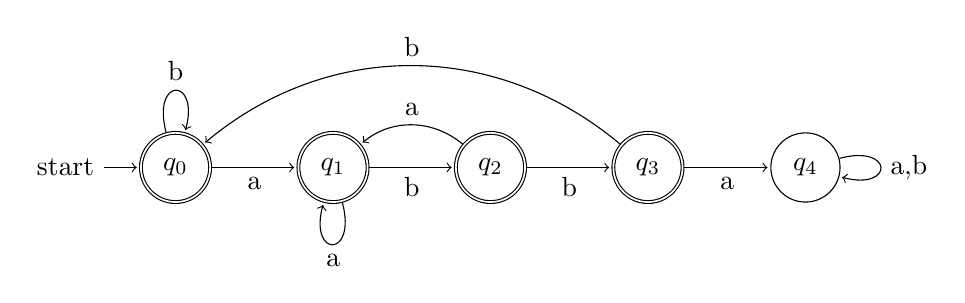
\begin{tikzpicture}[shorten >=1pt,node distance=2cm,on grid,auto]
      \node[state,initial, accepting] (q_0) {$q_0$};
      \node[state, accepting] (q_1) [right=of q_0] {$q_1$};
      \node[state, accepting] (q_2) [right=of q_1] {$q_2$};
      \node[state, accepting] (q_3) [right=of q_2] {$q_3$};
      \node[state] (q_4) [right=of q_3] {$q_4$};
      \path[->]
      (q_0) edge [loop above] node [above] {b} ()
        edge node [below] {a} (q_1)
      (q_1) edge node [below] {b} (q_2)
            edge [loop below] node [below] {a} ()
      (q_2) edge node [below] {b} (q_3)
            edge [bend right=40] node [above] {a} (q_1)
      (q_3) edge node [below] {a} (q_4)
            edge [bend right=40] node [above] {b} (q_0)
      (q_4) edge [loop right] node [right] {a,b} ();
    \end{tikzpicture}
  \end{quote}

  \clearpage

  \question{}\\\\\noindent\null\hspace{-4.3cm}
  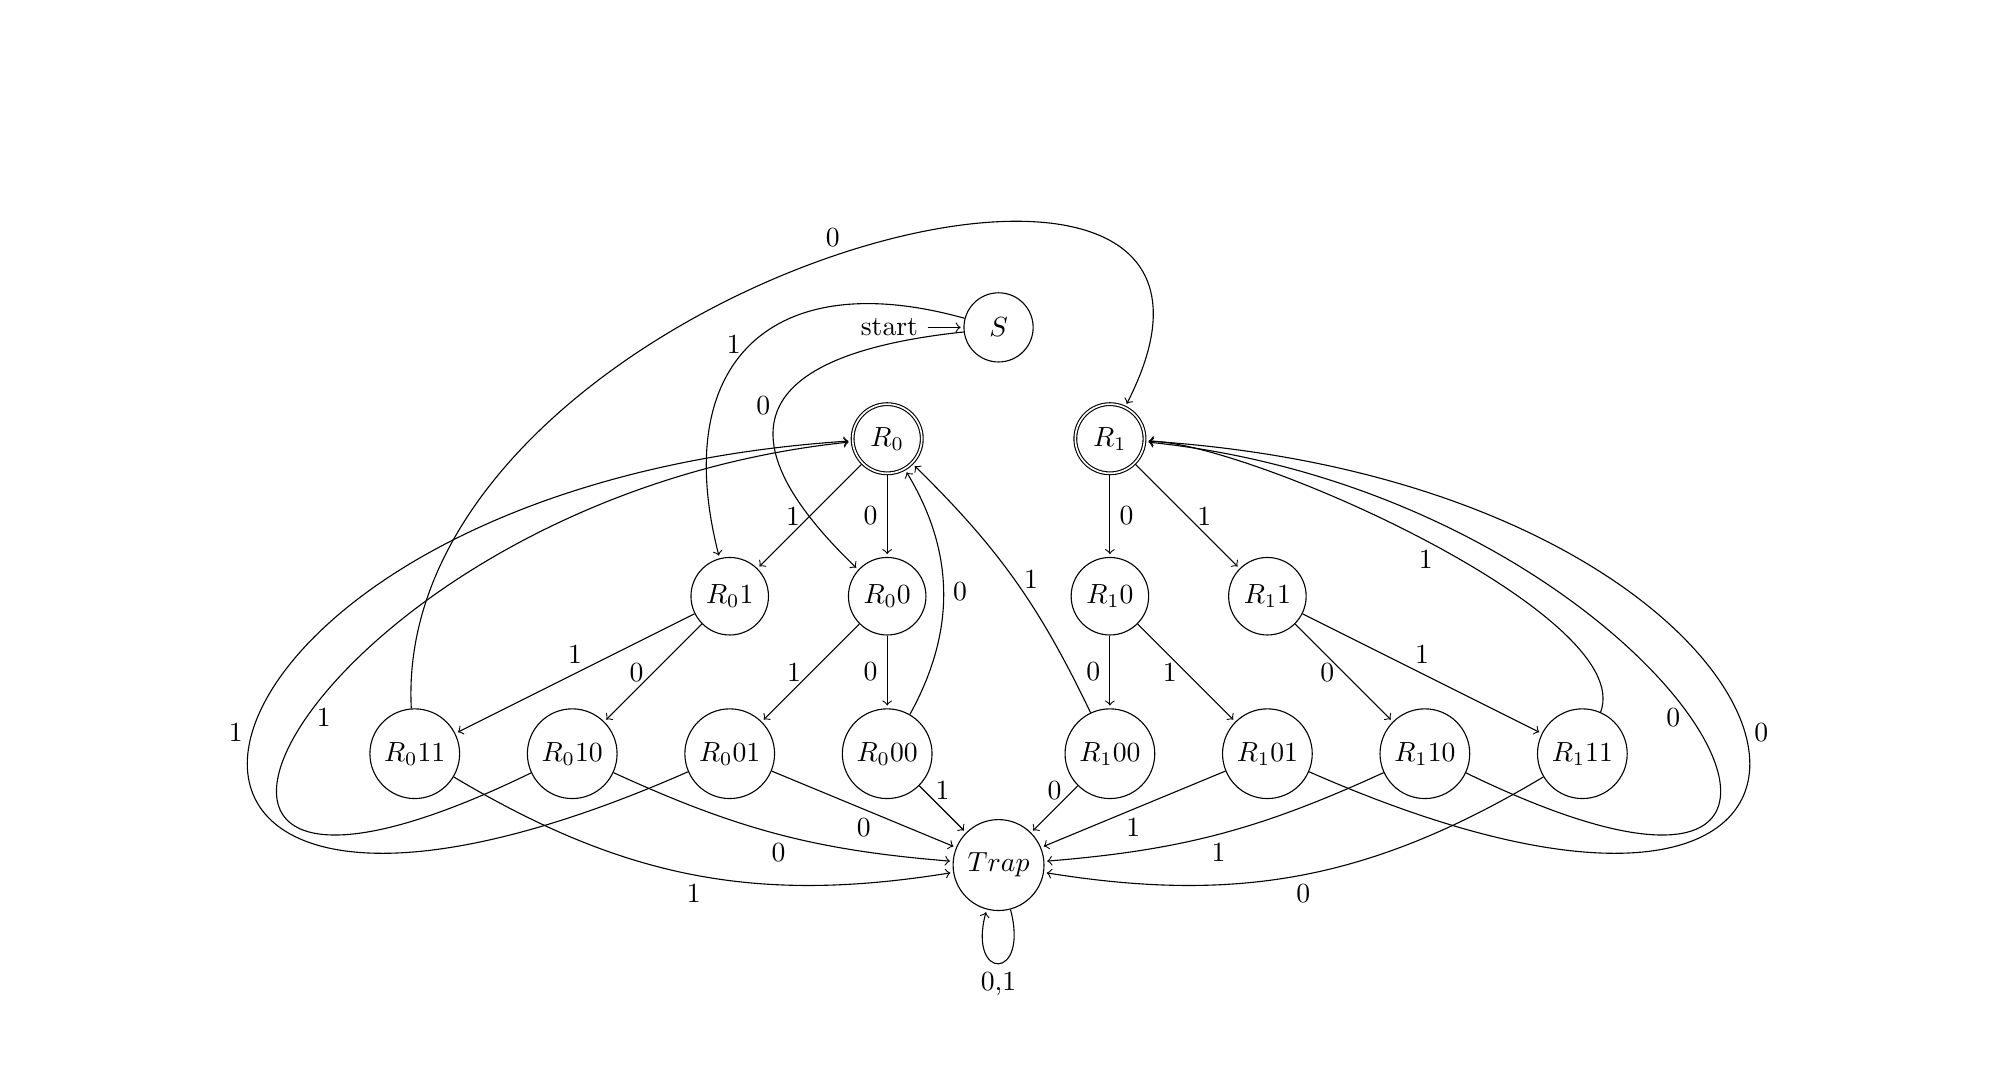
\begin{tikzpicture}[shorten >=1pt,node distance=2cm,on grid,auto]
    \node[initial, state] (q_0) {$S$};
    \node[state, accepting] (q_1) [below left= of q_0] {$R_0$};
      \node[state] (q_3) [below=of q_1] {$R_00$};
        \node[state] (q_5) [below=of q_3] {$R_000$};
        \node[state] (q_6) [left=of q_5] {$R_001$};
      \node[state] (q_4) [left=of q_3] {$R_01$};
        \node[state] (q_7) [left=of q_6] {$R_010$};
        \node[state] (q_8) [left=of q_7] {$R_011$};
    \node[state, accepting] (q_2) [below right=of q_0] {$R_1$};
      \node[state] (q_9) [below=of q_2] {$R_10$};
        \node[state] (q_11) [below=of q_9] {$R_100$};
        \node[state] (q_12) [right=of q_11] {$R_101$};
      \node[state] (q_10) [right=of q_9] {$R_11$};
        \node[state] (q_13) [right=of q_12] {$R_110$};
        \node[state] (q_14) [right=of q_13] {$R_111$};
    \node[state] (q_15) [below right=of q_5] {$Trap$};
    \path[->] (q_0) edge [bend right=40, looseness = 2, in=250, out=300] node [left] {0} (q_3)
                    edge [bend right=60, looseness=1.5] node [left] {1} (q_4);
    \path[->] (q_1) edge node [left] {0} (q_3)
                    edge node [left] {1} (q_4);
    \path[->] (q_2) edge node [right] {0} (q_9)
                    edge node [right] {1} (q_10);
    \path[->] (q_3) edge node [left] {0} (q_5)
                    edge node [left] {1} (q_6);
    \path[->] (q_4) edge node [left] {0} (q_7)
                    edge node [above] {1} (q_8);
    \path[->] (q_5) edge [bend right=30] node [right] {0} (q_1)
                    edge node [above] {1} (q_15);
    \path[->] (q_6) edge [bend right=30, out=140, in=120, looseness=5] node [left] {1} (q_1)
                    edge node [below] {0} (q_15);
    \path[->] (q_7) edge [bend right=30, out=160, in=140, looseness=3] node [right] {1} (q_1)
                    edge [bend right=10] node [below] {0} (q_15);
    \path[->] (q_8) edge [bend right=30, out=70, in=40, looseness=1.4] node [above] {0} (q_2)
                    edge [bend right=20] node [below] {1} (q_15);
    \path[->] (q_9) edge node [left] {0} (q_11)
                    edge node [left] {1} (q_12);
    \path[->] (q_10) edge node [left] {0} (q_13)
                    edge node [above] {1} (q_14);
    \path[->] (q_11) edge [bend right=10] node [right] {1} (q_1)
                    edge node [above] {0} (q_15);
    \path[->] (q_12) edge [bend right=30, out=220, in=240, looseness=5] node [right] {0} (q_2)
                     edge node [below] {1} (q_15);
    \path[->] (q_13) edge [bend right=30, out=200, in=220, looseness=3] node [left] {0} (q_2)
                     edge [bend left=10] node [below] {1} (q_15);
    \path[->] (q_14) edge [bend right=30, out=280, in=210, looseness=.5] node [below] {1} (q_2)
                     edge [bend left=20] node [below] {0} (q_15);
    \path[->] (q_15) edge [loop below] node [below] {0,1} ();
  \end{tikzpicture}



\end{document}
